\documentclass[12pt,english]{article}

\usepackage[a4paper,
            bindingoffset=0.2in,
            left=1in,
            right=1in,
            top=1in,
            bottom=1in,
            footskip=.25in]{geometry}

% % Set page size and margins
% % Replace `letterpaper' with`a4paper' for UK/EU standard size
% \usepackage[letterpaper,top=2cm,bottom=2cm,left=3cm,right=3cm,marginparwidth=1.75cm]{geometry}
\topmargin=-.3in \oddsidemargin=.3in \evensidemargin=.3in \textheight=9in \textwidth=6in

\usepackage{tikz}
\usepackage{pgfplots}
\usepackage{float}
\usepackage{adjustbox}
\usepackage{multirow}
\usepackage{hhline}

\usepackage{algorithm, algpseudocode}
\usepackage{setspace}

\algrenewcommand\textproc{}

\algnewcommand\algorithmicswitch{\textbf{switch}}
\algnewcommand\algorithmiccase{\textbf{case}}
\algnewcommand\algorithmicassert{\texttt{assert}}
\algnewcommand\Assert[1]{\State \algorithmicassert(#1)}%
% New "environments"
\algdef{SE}[SWITCH]{Switch}{EndSwitch}[1]{\algorithmicswitch\ #1\ \algorithmicdo}{\algorithmicend\ \algorithmicswitch}%
\algdef{SE}[CASE]{Case}{EndCase}[1]{\algorithmiccase\ #1}{\algorithmicend\ \algorithmiccase}%
\newcommand{\pluseq}{\mathrel{{+}{=}}}
\algblockdefx[Foreach]{Foreach}{EndForeach}[1]{\textbf{foreach} #1 \textbf{do}}{\textbf{end foreach}}


% \newcommand{\makeheight}[1]{%
%   \settoheight{\dimen0}{T}% a capital letter
%   \rule[-\dimexpr(#1-\dimen0)/2]{0pt}{#1}%
% }

\newcommand{\myindent}[1]{
\newline\makebox[#1cm]{}
}

\usepackage{amsmath}

\usepackage{pdfpages}



\title{\textbf{Appendix}}
\date{}

\begin{document}
\maketitle

\section{Cut Isnad to Individual Transmissions}
\begin{center}
\begin{minipage}{.8\linewidth}
\begin{algorithm}[H]
\setstretch{1}
\caption{Cut Isnad to Individual Transmissions}\label{euclid}
\begin{algorithmic}[1]
\Require isnad, edge\_list
\State \textit{cut\_isnad} $\gets$ \{value: isnad text for individual transmissions\}
\Foreach{\text{edge} $\in$ \text{edge\_list}}
\State teacher\_id, student\_id $\gets$ edge[0], edge[1]
\State beg\_string, end\_string $\gets$ ``L\#" + \textbf{toString}(teacher\_id), \myindent{4.9} ``L\#" + \textbf{toString}(student\_id)
\State transmission\_text $\gets$ string match from beg\_string to \myindent{4.17} end\_string
\State cut\_isnad.\textbf{append}(transmission\_text)
\EndForeach
% \State return \textit{time}
\end{algorithmic}
\end{algorithm}
\end{minipage}
\end{center}

\newpage
\section{Build MoT Corpus} % example of a heading
\begin{center}
\begin{minipage}{.8\linewidth}
\begin{algorithm}[H]
\setstretch{1}
\caption{Build MoT Corpus}\label{euclid}
\begin{algorithmic}[1]
\Require cut\_isnads
\State \textit{mot\_corpus} $\gets$ \{value: MoT words
\}
\State mot\_corpus $\gets$ initialize corpus with $\alpha$ MoT words  \texttt{\small{/* Where $\alpha$ \myindent{2.3} is the number of known MoT words */}}
\State need\_investigation = \{value: transmission text\}
\Foreach{\text{transmission\_text} $\in$ \text{cut\_isnads}}
    \State matched\_mot $\gets$ False
    \Foreach{\text{mot} $\in$ \text{mot\_corpus}}
        \If{mot in transmission\_text}
            \State matched\_mot = True
            \State \textbf{break}();
        \EndIf 
    \EndForeach
    \If{not matched\_mot}
         \State need\_investigation.\textbf{append}(transmission\_text);   
    \EndIf 
\EndForeach
\If{\textbf{len}(need\_investigation) $==$ 0}
    \State \texttt{\small{/* manually look at $\beta$ transmissions in \myindent{.85} need\_investigation and add the undidentifed MoT \myindent{.85} words to the $\alpha$ known ones */}}
    \State \texttt{\small{/* repeat process until need\_investigation is empty */}}
\EndIf 
\end{algorithmic}
\end{algorithm}
\end{minipage}
\end{center}

\newpage
\section{Extract MoT from Cut Isnad Tranmissions} % example of a heading
\begin{center}
\begin{minipage}{.8\linewidth}
\begin{algorithm}[H]
\setstretch{1}
\caption{Extract MoT from Cut Isnad Tranmissions}\label{euclid}
\begin{algorithmic}[1]
\Require mot\_corpus, cut\_isnads
\State \textit{transmission\_mot} = \{value: \textbf{pair}(transmission, mot)\}
\Foreach{\text{transmission} $\in$ \text{cut\_isnads}}
    \State matched\_mots $\gets$ \{value: \textbf{pair}(mot, position)\}
    \Foreach{\text{mot} $\in$ \text{mot\_corpus}}
        \If{mot in transmission}
            \State position $\gets$ position of mot in transmission
            \State matched\_mots.\textbf{append}((mot, position))
        \EndIf 
    \EndForeach
    \State selected\_mot $\gets$ apply heuristics to select mot from \myindent{3.35} matched\_mots
    \State transmission\_mot.\textbf{append}(\textbf{pair}(transmission, \myindent{6.25} selected\_mot))
\EndForeach

\end{algorithmic}
\end{algorithm}
\end{minipage}
\end{center}

\newpage
\section{Transmission Time}
\begin{center}
\begin{minipage}{.8\linewidth}
\begin{algorithm}[H]
\setstretch{1}
\caption{Place Transmission in Time Span}\label{euclid}
\begin{algorithmic}[1]
\Require teacher\_bio, student\_bio
\State const\_lifespan = 80
\State const\_childhood = 20
\State death\_date\_teacher $\gets$ death date from  teacher\_bio
\State death\_date\_student $\gets$ death date from student\_bio
\If{birth\_date $\in$ teacher\_bio}
    \State birth\_date\_teacher $\gets$ birth date from  teacher\_bio
\Else
    \State birth\_date\_teacher $\gets$ death\_date\_teacher \myindent{4.2} $-$  const\_lifespan
\EndIf 
\If{birth\_date $\in$ student\_bio}
    \State birth\_date\_teacher $\gets$ birth date from student\_bio
\Else
    \State birth\_date\_student $\gets$ death\_date\_student \myindent{4.2} $-$ const\_lifespan
\EndIf 
\State upper\_bound $\gets$ \textbf{min}(death\_date\_teacher, death\_date\_student)
\State lower\_bound $\gets$ \textbf{max}(birth\_date\_teacher, birth\_date\_student)
% \EndProcedure
\If{upper\_bound $-$ lower\_bound $>$ const\_childhood}
    \State lower\_bound $\mathrel{+}=$ const\_childhood
\EndIf 
\State \textit{time\_span} $\gets$ (lower\_bound, upper\_bound)
% \State return \textit{time}
\end{algorithmic}
\end{algorithm}
\end{minipage}
\end{center}

\begin{figure}
   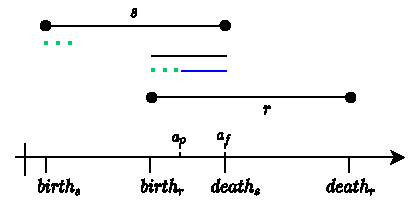
\includepdf[scale=0.5,offset=0 -175]{testing4.pdf}
\end{figure}

\end{document}